\chapter{Problem Specification}

In this chapter we will introduce the graph optimisation problem and establish the baseline performance using cost-based backtracking optimisation. Next, we will frame the optimisation problem in the RL domain by describing the system environment, the reward calculation and the state-action space. Additionally, we describe the RL agents trained in the model-free and model-based domains and we also highlight limitations in the application of reinforcement learning to this problem.

\section{Introduction}
The major deep learning frameworks such as TensorFlow \cite{tensorflow2015-whitepaper} and PyTorch \cite{pytorch} used greedy rule-based graph transformation prior to execution. Furthermore, in Chapter \ref{sec:bg:subsec:currentapp} we described the prior work upon which this work builds. Namely, we introduced the work by Jia et al. \cite{jia2019taso,jia2019optimizing} that proposed an approach for performing an offline optimisation of deep learning computation graphs using a recursive backtracking search in the action space. Specifically, the authors developed a framework that uses a pre-generated set of formally verified, semantically equivalent graph substitutions that can be used to modify the graph to search for a reduced runtime.

\section{Optimisation of deep learning graphs}

TensorFlow (TF) uses a system called \textit{``Grappler''} that is the default graph optimisation system in the TF runtime \cite{larsen2019tensorflow}. By natively performing the graph optimisation at runtime, it allows for a interoperable, transparent optimisation strategy via protocol buffers. To improve the performance of the underlying model, Grappler supports a range of features such as the pruning of dead nodes, removal of redundant computation and improved memory layouts. Concretely, Grappler was designed with three primary goals:

\begin{itemize}
  \item Automatically improve performance through graph simplifications and high-level optimisations to benefit the most target architectures
  \item Reduce device peak memory usage
  \item Improve hardware utilisation by optimising device placement
\end{itemize}

On the other hand, although Grappler can automatically optimise the data-flow graphs of deep learning models, such a complex optimisation system presents challenges. Firstly, significant engineering effort is required to implement, verify and test the optimiser to ensure the correctness of the graph rewrites rules; TF contains a set of 155 substitutions that are implemented in 53,000 lines of code; to further complicate matters, new operators are continuously proposed, such as grouped or transposed convolutions, all of which leads to a large amount effort expended to maintain the library. Secondly, and perhaps more importantly, as TF uses Grappler at runtime by default, it adds overhead to execution as extra graph conversions are performed at runtime rather than offline.

\begin{figure}[ht]
  \centering
  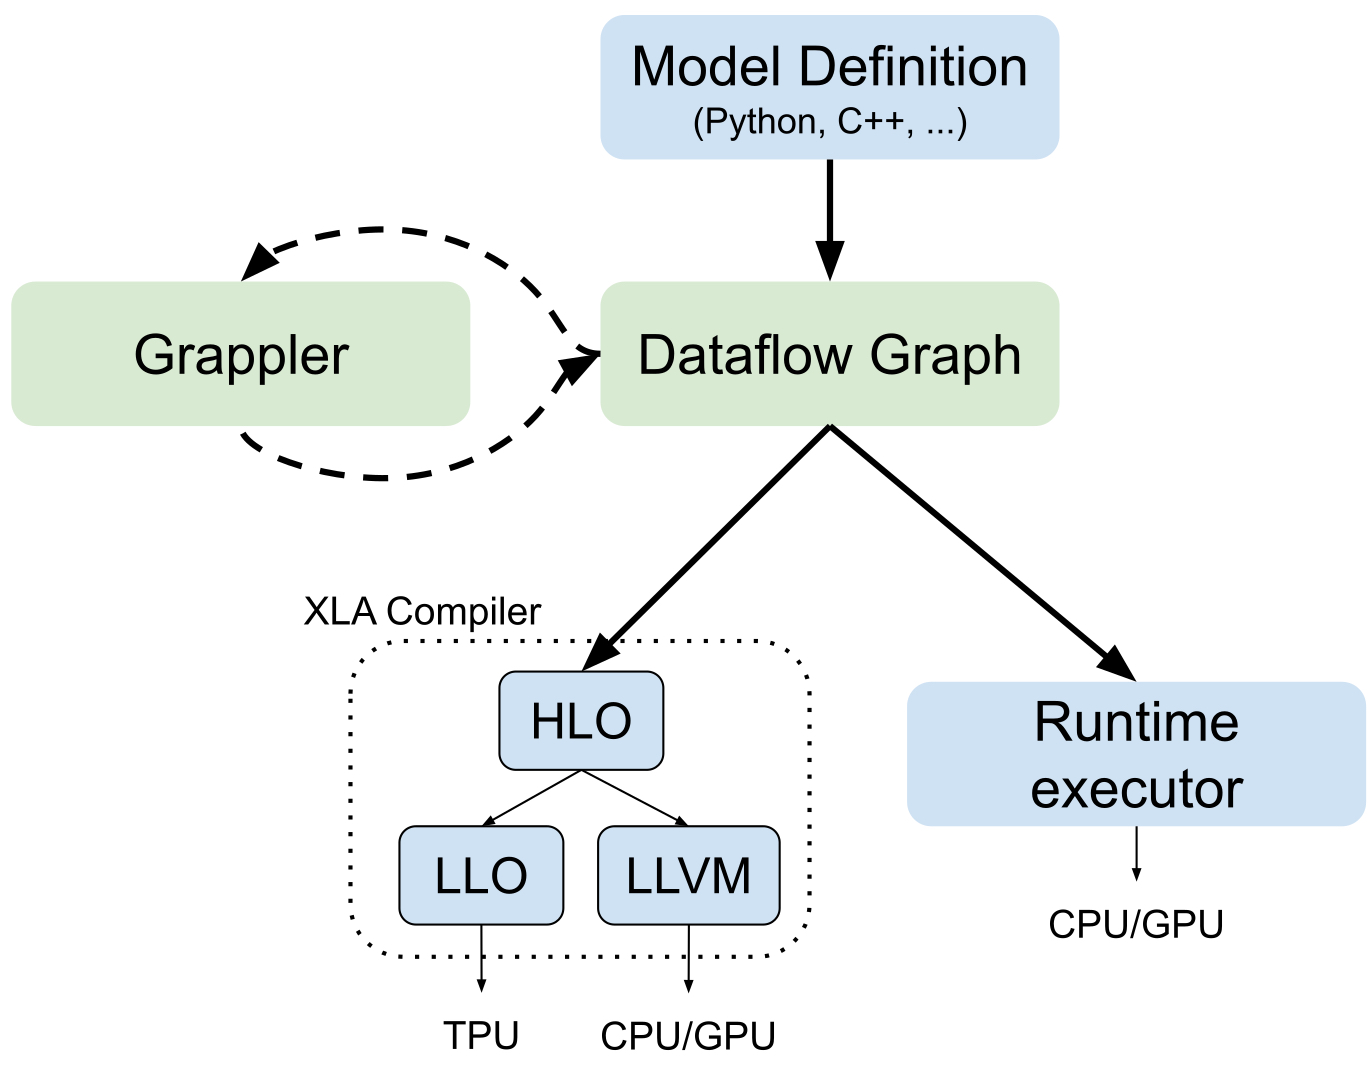
\includegraphics[width=0.75\columnwidth]{sections/3problem/images/GraphOptimiser.jpg}
  \caption[Architecture of graph optimisation system in TensorFlow]{The machine learning model is processed prior to execution by either Grappler, the static graph optimiser in TensorFlow, or via JIT compilation of the model using XLA. Figure adapted from \cite{larsen2019tensorflow}.}
  \label{fig:problem:graph-optim}
\end{figure}

Alternatively, both TensorFlow, and more recently PyTorch, support automatic graph optimisation by JIT (just-in-time) compilation through XLA and the \texttt{torch.jit} package respectively. In Figure \ref{fig:problem:graph-optim} we can see a high-level view of the components of the optimisation system. In order to motivate the reasoning to perform offline optimisation rather than JIT optimisation we  consider the work proposed by Jia et al. in both MetaFlow and TASO, the systems they design can be used as a drop-in replacement of the Grappler and/or XLA compilation steps.

TASO applies all possible candidate transformations at each step and estimates the runtime (or cost) of the final graph. Next, TASO chooses the highest performing candidates for the proceeding iteration of candidate evaluations. Principally, this approach is superior to the naive greedy optimisation approach as we can use the estimated runtime to guide the search and forego immediate improved runtime to increase the potential search space of candidate graphs.

In addition, as TASO operates at the graph-level, its optimisations are completely orthogonal to operator-level optimisations; thus it can be combined with code generation techniques such as TVM \cite{chen2018tvm} or Astra \cite{sivathanu2019astra} to further improve overall performance. We also note that TASO performs tensor data layout and graph transformation simultaneously rather than sequentially. It has been shown that by considering it as a joint optimisation problem end-to-end inference runtime can be reduced by up to 1.5x \cite{jia2019taso, jia2019optimizing}.

% However, using estimated runtime presents a challenge with respect to the exponential growth of search space at a rate of $O(N^T)$, where $N$ is the number of transformations and $T$ is the number of search steps.

\subsection{Graph-level optimisation}

Performing optimisations at a higher, graph-level means that the resulting graph is - in terms of execution methodology - no different than the original graph prior to optimisation. Therefore, by performing graph-level optimisation we generate a platform and backend independent graph representation which can be further optimised by specialised software for custom hardware accelerators such as GPUs and TPUs.

Next, we define that two computation graphs, $\mathcal{G}$ and $\mathcal{G}'$ are semantically equivalent when $\forall \mathcal{I} : \mathcal{G}(\mathcal{I}) = \mathcal{G}'(\mathcal{I})$ where $\mathcal{I}$ is an arbitrary input tensor. We aim to find the optimal graph $\mathcal{G}^*$ that minimises the cost function, \texttt{cost}$(\mathcal{G})$, by performing a series of transformations to the computation graph - at each step, the specific transformation applied does not need to be strictly optimal. In fact, by applying optimisations that reduce graph runtime we further increase the state space for the search; a large state space is preferable in the reinforcement learning domain.

An important problem in graph-level optimisation is that of defining a set of varied, applicable transformations that can be used to optimise the graphs. As previously noted, prior work such as TensorFlow use a manually defined set of transformations and optimise greedily. On the other hand, TASO uses a fully automatic method to generate candidate transformations by performing a hash-based enumeration over all possible DNN operators that result in a semantically equivalent computation graph.

\begin{figure}[ht]
  % preliminary
  \sbox\twosubbox{%
    \resizebox{\dimexpr.9\textwidth-1em}{!}{%
      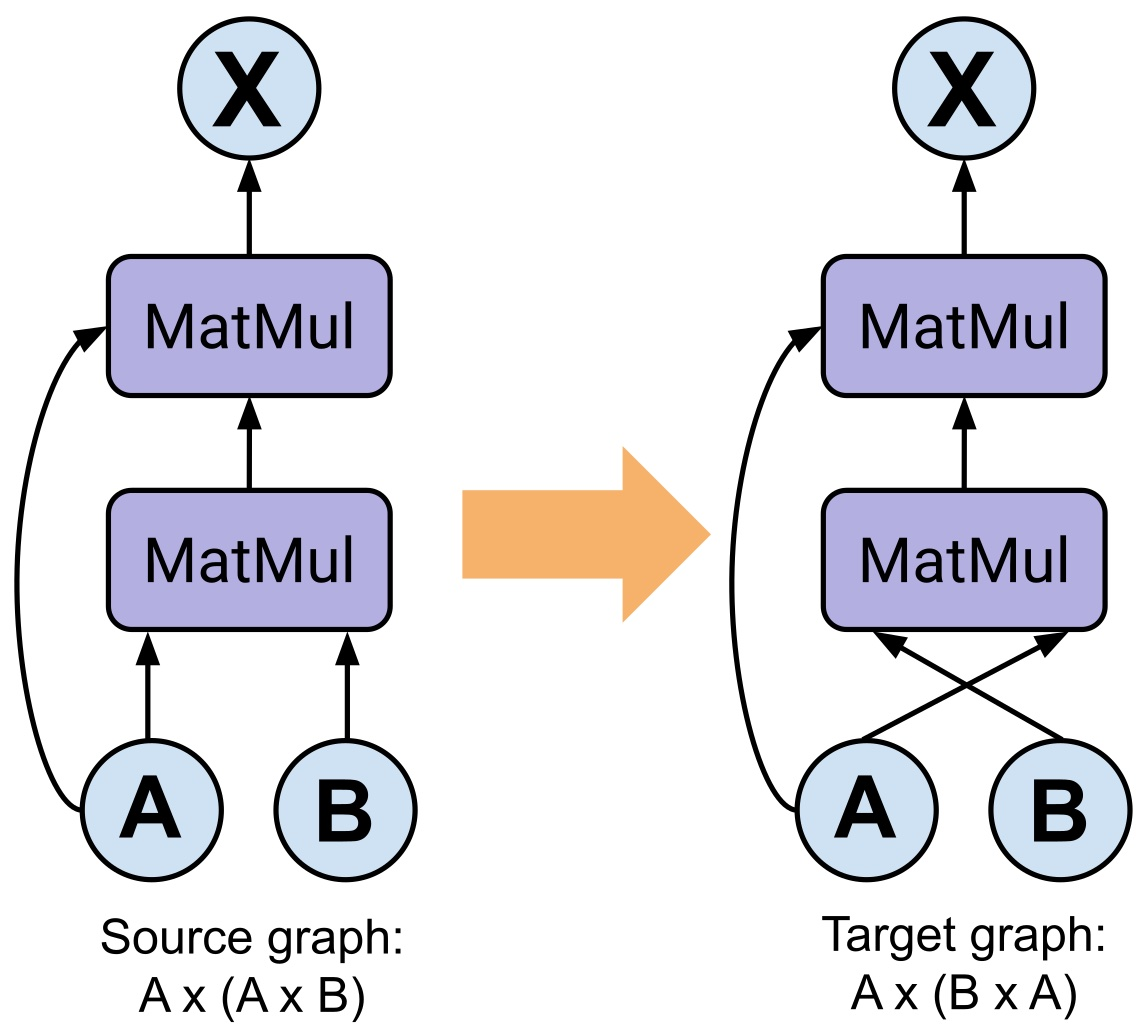
\includegraphics[height=3cm]{sections/3problem/images/rewrite1.jpg}%
      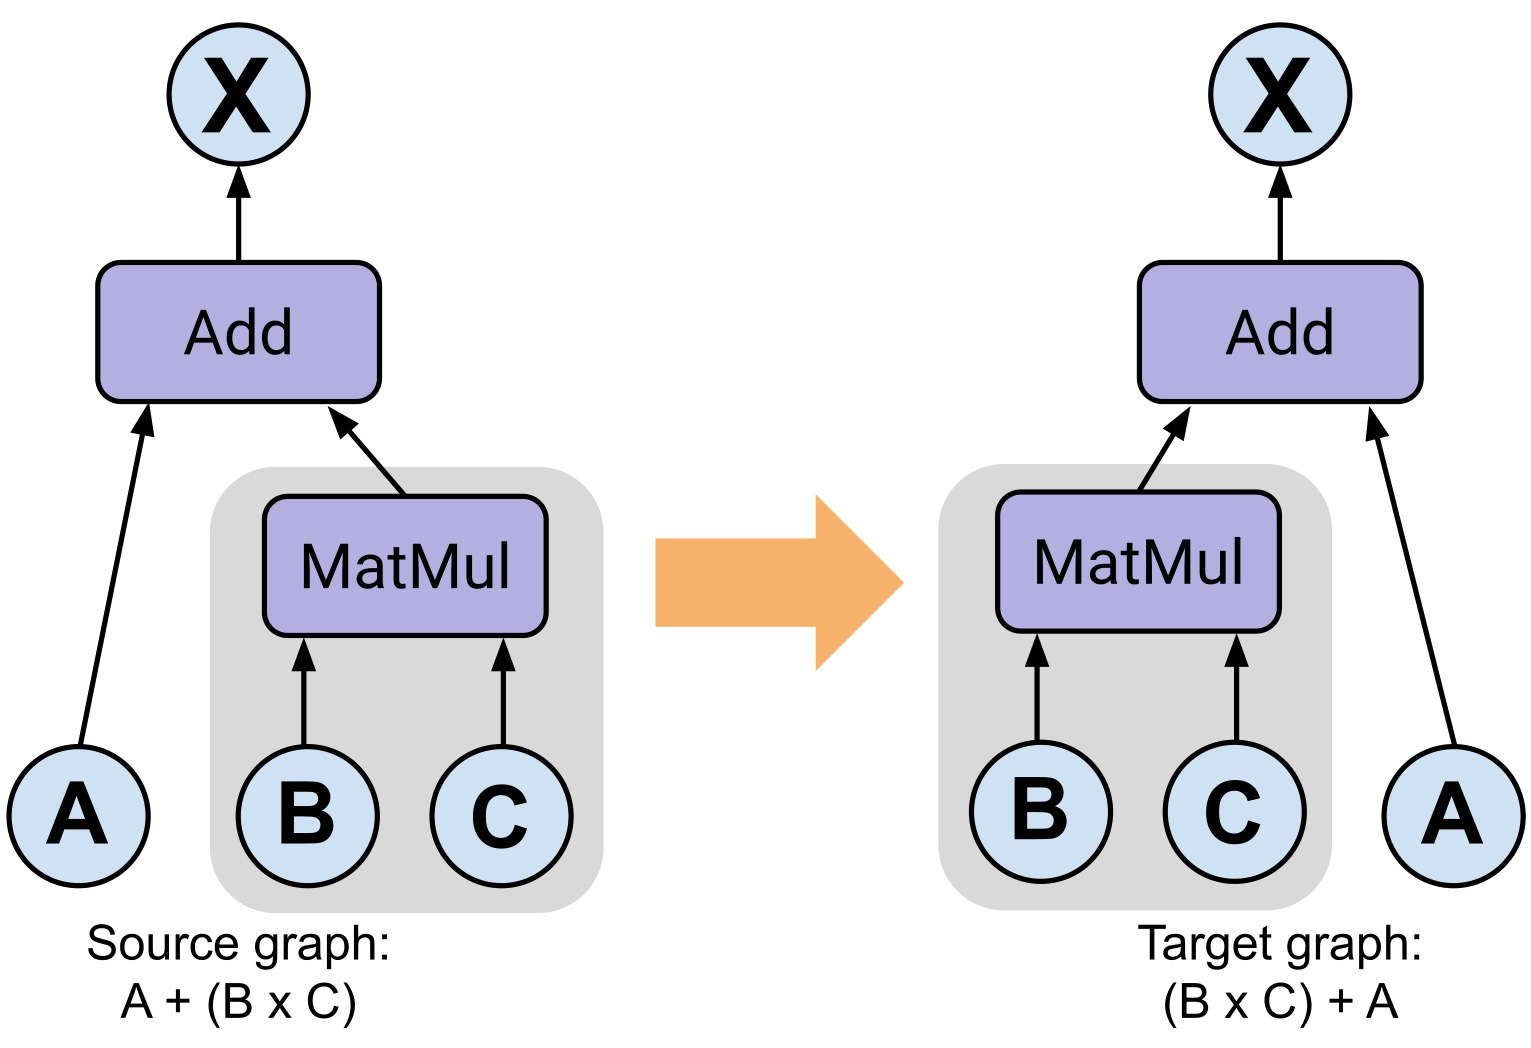
\includegraphics[height=3cm]{sections/3problem/images/rewrite2.jpg}%
    }%
  }
  \setlength{\twosubht}{\ht\twosubbox}
  
  % typeset
  \centering
  \subcaptionbox{Tensor renaming substitution \label{fig:problem:rewrite-graph1}}{
    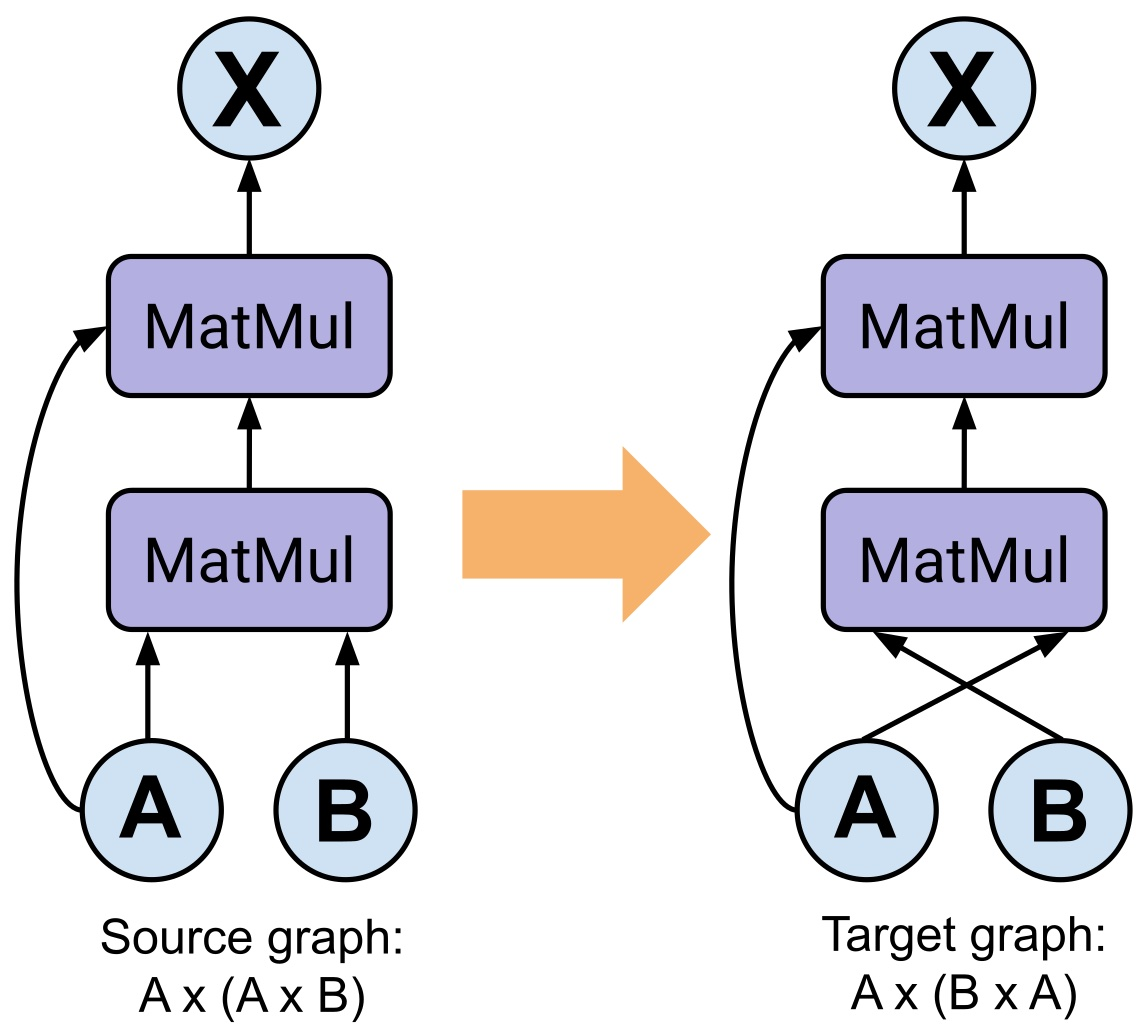
\includegraphics[height=\twosubht]{sections/3problem/images/rewrite1.jpg}
  }\quad
  \subcaptionbox{Common subgraph substitution \label{fig:problem:rewrite-graph2}}{
    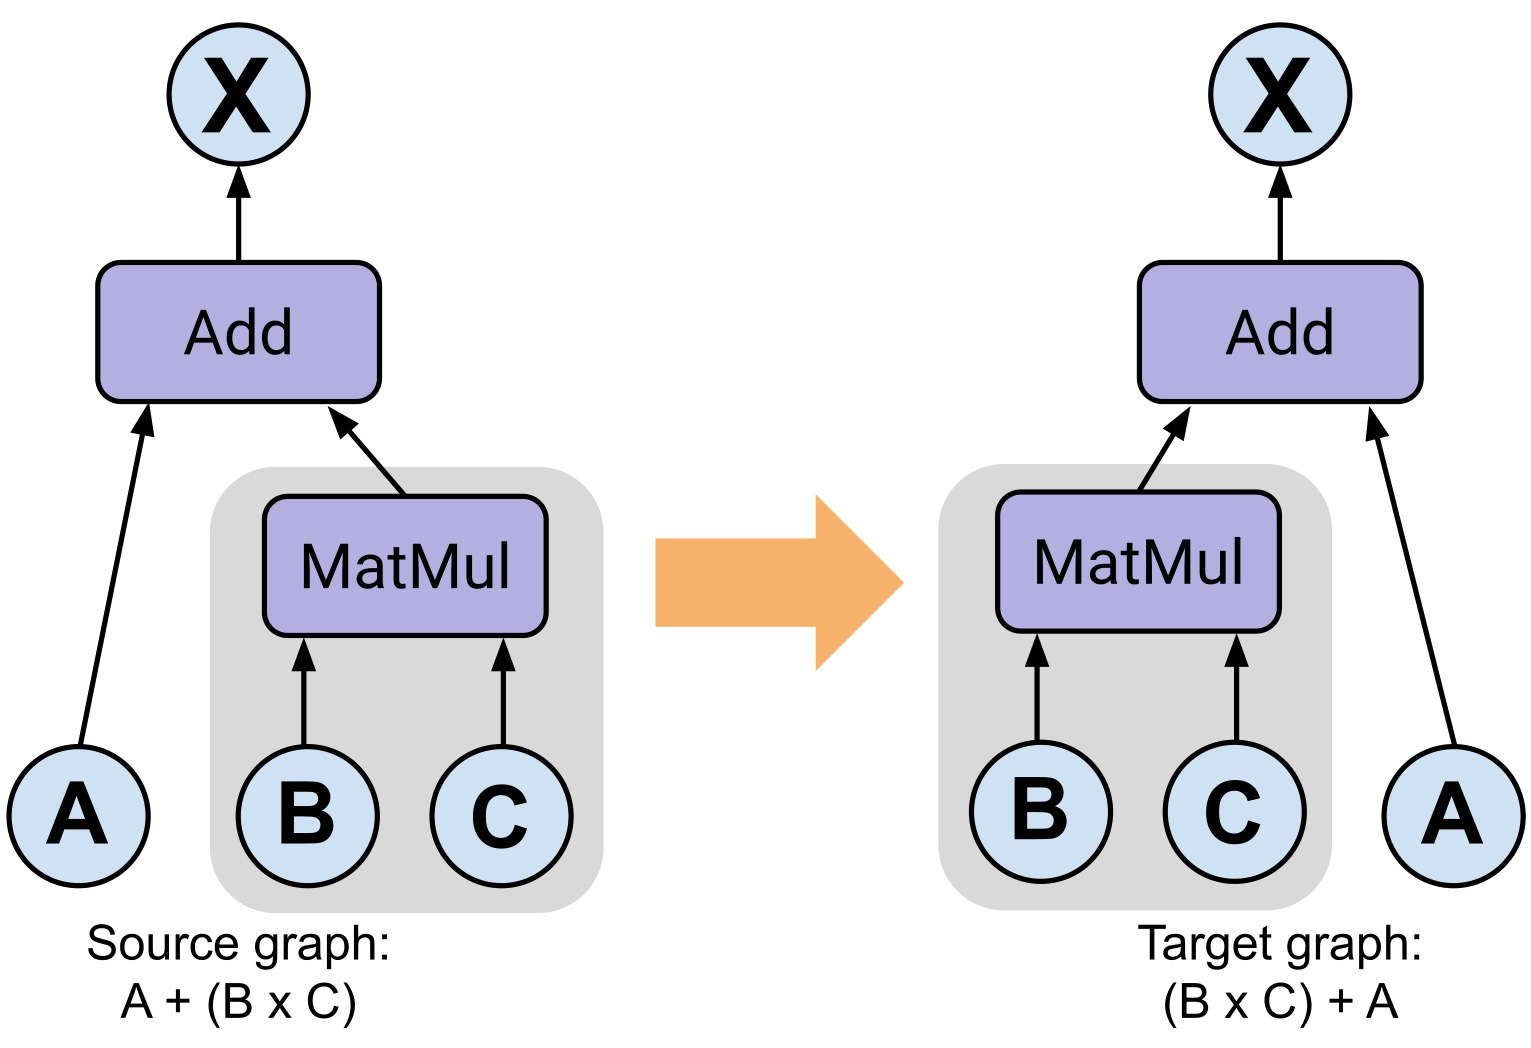
\includegraphics[height=\twosubht]{sections/3problem/images/rewrite2.jpg}
  }
  \caption[Two examples of trivial graph substitutions]{Two examples of trivial graph substitutions that does not impact the overall runtime of the computation graph. The left sub-figure shows a simple renaming of the tensor inputs. The figure on the right shows that we have a common sub-graph between the source and the target graphs. In both cases we eliminate the duplicates as the hash of the two graphs will be identical.}
\end{figure}

In this work, we take the same approach as that of TASO and automatically generate the candidate graphs. We perform this as an offline step as it requires a large amount of computation to both generate and verify the candidate substitution; to place an upper bound on the computation, we limit the input tensor size to a maximum of 4x4x4x4 during the verification process. Following the generation and verification steps, we prune the collection to remove substitutions that are considered trivial and as such would not impact runtime. For example, trivial substitutions include input tensor renaming and common subgraphs, we show both techniques diagrammatically in Figure \ref{fig:problem:rewrite-graph1} and \ref{fig:problem:rewrite-graph2} respectively.

- TODO: TASO algo for searching for optimal graph

\subsection{Baselines}
In order to establish a baseline performance measure for performing graph-level optimisation of deep learning models we have two different sources. Firstly, we can measure the performance of a select number of deep learning models in the standard DL frameworks, TensorFlow and PyTorch. In this project, there are common, standardised mechanisms for evaluating the performance of models using these frameworks - we show the results of the baseline measurements in the following section.

Secondly, in this work, we replicate the experiments as performed by Jia et al. \cite{jia2019taso} and use the results as our benchmark to compare our work against. However, for the majority of evaluated graphs we used a lower budget than that of the authors in the original paper. We found that using a lower search budget, without alteration of the hyperparameter $\alpha$, it did not result in a lower performance compared to the original experiments. Figure [TODO] shows the results of the heuristic search for the graph $\mathcal{G}^*$ and Figure [TODO] shows the relative performance of the methods on each chosen deep learning model. 

% {\SetAlgoNoLine
\begin{algorithm}[H]
 \setstretch{1.0}
 \textbf{Input}: Initial computation graph $\mathcal{G}_0$, a cost function \texttt{cost}($\mathcal{G}$), a list of valid graph substitutions $\lbrace S_1, \dots, S_m$, and the hyperparameter $\alpha$ \\

 \textbf{Output}: An optimised computation graph $\mathcal{G}^*$

 \texttt{//} $\mathcal{Q}$ is a priority queue of graphs sorted under \texttt{cost}.\\
 $\mathcal{Q} = \lbrace \mathcal{G}_0 \rbrace$

 \While{$\mathcal{Q} \neq \lbrace \rbrace$}{
   $\mathcal{G} = \mathcal{Q}$.\texttt{dequeue()}\\
   \For{$i = 1 \dots m$}{
    $\mathcal{G}' = S_i(\mathcal{G})$ \\
    \If{\texttt{cost}($\mathcal{G}'$) $<$ \texttt{cost}($\mathcal{G}^*$)}{
      $\mathcal{G}^* = \mathcal{G}'$
    }
    \If{\texttt{cost}($\mathcal{G}'$) $< \alpha~\times$ \texttt{cost}($\mathcal{G}^*$)}{
      $\mathcal{Q}$.\texttt{enqueue($\mathcal{G}'$)}
    }
  }
 }
 \Return{$\mathcal{G}^*$}

 \caption{Cost-based backtracking search. Adapted from \cite{jia2019taso}.}
 \label{algo3}
\end{algorithm}}

% - Estimation of runtime characteristics for each tensor op --> imperfect estimation

% - Using real runtime is difficult as it takes longer to simulate and large variation in measurements between runs

\section{Reinforcement Learning formulation}
In the following section we will describe how to represent the computation graph optimisation problem in the reinforcement learning domain by describing the key components of the system. We describe the system environment in which the agents act, the state-action space, and finally the reward functions for both the model-free and model-based agents which we used to determine the optimal reward signal to train the agents.

\subsection{System environment}

In order to train a reinforcement learning agent, it necessary that we have access to an environment that, given the current environment state, the agent can take an action. After taking the chosen action, the environment is updated into a new state and the agent receives a reward signal. Typically, one uses a mature environment such as OpenAI Gym \cite{brockman2016openai} or OpenSpiel \cite{LanctotEtAl2019OpenSpiel} as the quality of the environment often has a significant effect on the stability of training. Moreover, using an environment that uses a common interface allows researchers to implement algorithms with ease and, importantly, reproduce results from published conference papers.

In our work, we implemented an environment that follows the OpenAI Gym API standard stepping an environment, that is, we have a function \texttt{step(action)} that accepts a single parameter, the action requested by the agent to be performed in the environment. The \texttt{step} function returns a 4-tuple \texttt{(next\textunderscore state, reward, terminal, extra\textunderscore info)}. \texttt{extra\textunderscore info} is a dictionary which can store arbitrary data. The environment in our project has a structure that is shown diagrammatically in Figure [TODO].

To simplify the implementation of the environment, we used made extensive use of the work by Jia et al. \cite{jia2019taso} with the open source version of TASO. We provide a computation graph and the chosen transformation and location; TASO then applies the requested transformation and returns the newly transformed graph. Further, we use internal TASO functions that calculates estimates of the runtime on the hardware device which we use as our reward signal for training the agent. During our experiments we modified TASO to extract detailed runtime measurements to analyse the rewards using a range of different reward formulae - we describe our approach further in section \ref{sec:prob:subsec:rwd}.

The scope of our work meant that there was no existing prior work that applied reinforcement learning to the task of optimising deep learning computation graphs. Thus, we required an environment in which an agent can act efficiently. Due to the nature of systems environments, the interactions with the real-world environment can be often slow, especially compared to those such as Arcade Learning Environment \cite{Bellemare_2013}. An aim of this work was to train a simulated environment, a ``world model'', that if accurate in relation to the real environment, we can train an agent far more efficiently than would be possible with the real-environment. In section [TODO] we will further explore world models and evaluate our implementation.

\subsection{State-Action space}
In this project we modelled the state and action space in accordance with prior research, specifically we referenced work in a similar domain of system optimisation using reinforcement learning; Mirhoseini et al. \cite{mirhoseini2018hierarchical} used hierarchical RL with multiple actions to find the optimal device placement and Addanki et al. \cite{addanki2019placeto} that also aided in the design choice of input/output graph sizes.

Next, we require two values in order to update the environment. First, we need a select a transformation (which we refer to as an \texttt{xfer}) to apply to the graph. Secondly, the location at which to apply the transformation. As we need to select two actions that are dependent on each other to achieve a higher performance, it requires selecting the actions simultaneously.

However, this would require a model output of $N \times L$ values, where $N$ is the number of transformations, $L$ is the number of locations. Such an action space is too large to train a model to efficiently predict the correct action. Additionally, after choosing a transformation, we ideally mask the available locations as not all locations can be used to apply a transformation. Therefore, using the same trunk network, we first predict the transformation, apply the location mask for the selected transformation, then predict the location.

We define the action as 2-value tuple of (xfer\textunderscore id, location). There is a special case for the xfer\textunderscore id. When it equals N (the number of available transformations), we consider it the NO-OP action. Therefore, in this special case we do not modify the graph, rather we terminate the current episode and reset the environment to its initial state.

As explained in the previous section, we used an step-wise approach where at each iteration, we provide a 2-tuple of the transformation and location, to apply in the current state. The updated state from the environment is a 4-tuple consisting of \texttt{(graph\textunderscore tuple, xfer\textunderscore tuples, location\textunderscore masks, xfer\textunderscore mask)}.

\texttt{xfer\textunderscore mask} refers to a binary mask that indicates the valid and invalid transformations that can be applied to the current computation graph as not every transformation can be applied to every graph. If the current graph has only four possible transformations that can be applied, all other transformations considered to be invalid. Thus, we return a boolean location mask where only valid transformations are set to 1, or \texttt{true}. This can be used to zero-out the model logits of invalid transformations (and thereby actions also) to make ensure the agent always selects a valid transformation from the set.

Similarly, for each transformation selected by the agent, there are a number of valid locations where this transformation can be applied. We set a hardcoded, albeit configurable, limit the number of locations to 200 in this work. If the current graph has fewer than 200 possible locations for any given transformation, the remaining are considered invalid. Therefore, we again return a boolean location mask, which is named \texttt{location\textunderscore masks} in the 4-tuple defined above, which can be used to zero out the model logits that which the locations are invalid. 

% We use the location masks for every transformation, therefore, we have a $N \times L$ tensor, where $N$ is the number of transformations, and $L$ is the maximum number of valid locations.

\subsection{Reward determination}
\label{sec:prob:subsec:rwd}
- Runtime difference

- Inclusion of detailed measurements

- Real-time measurements instead of estimated?

- Look up research on RL rewards (what makes a good reward signal)
